\documentclass[11pt]{article}
\usepackage[utf8]{inputenc}
\usepackage{amsmath, amssymb}
\usepackage{enumitem}
\usepackage{geometry}
\geometry{margin=1in}
\usepackage{hyperref}
\usepackage{color}
\usepackage{tcolorbox}
\usepackage{amsthm}
\usepackage{caption}
\usepackage{graphicx}

\theoremstyle{definition}
\newtheorem*{definition}{Definition}

\theoremstyle{remark}
\newtheorem*{remark}{Remark}

\theoremstyle{plain}
\newtheorem*{theorem}{Theorem}

\newtheoremstyle{solutionstyle} % Define a custom style
  {6pt}   % Space above
  {6pt}   % Space below
  {}      % Body font
  {0pt}      % Indent amount
  {\bfseries} % Theorem head font (bold)
  {.}     % Punctuation after theorem head
  {0.3em}   % Space after theorem head
  {}      % Theorem head specification

\theoremstyle{solutionstyle}
\newtheorem*{solution}{Solution}

\newtcolorbox{embox}{
    % colback=red!5!white,
    colframe=gray!75!black,
    % fonttitle=\bfseries,
    % title=Goal
}

\newtcolorbox{defbox}{
    colback=red!5!white,
    colframe=red!75!black,
    fonttitle=\bfseries,
    title=Definition
}

\newtcolorbox{algobox}{
    colback=blue!5!white,
    colframe=blue!75!black,
    fonttitle=\bfseries,
    title=Algorithm
}

\title{CS 3780 Notes}
\author{Jinzhou Wu}
\date{\today}

\begin{document}

\setcounter{tocdepth}{1}

\maketitle

\tableofcontents

\newpage

\section{Supervised Learning and KNN}
\textbf{Date:} \underline{Aug 28, 2025}

\subsection{Supervised Learning}

In supervised learning, we are given a dataset:
\[
S = \{ (x_1, y_1), (x_2, y_2), \dots, (x_n, y_n) \}
\]
where $x_i \in \mathcal{X}$ is a feature vector and $y_i \in \mathcal{Y}$ is its label.  
The goal is to learn a hypothesis function:
\[
h: \mathcal{X} \to \mathcal{Y}
\]
that approximates the unknown target function $f: \mathcal{X} \to \mathcal{Y}$.

\subsubsection*{Key Concepts}
\begin{itemize}
    \item \textbf{Instance:} A single feature vector $\mathbf{x} \in \mathcal{X}$.
    \item \textbf{Instance Space} $\mathcal{X}$: The set of all possible feature vectors.
    \item \textbf{Label} $y$: The output to be predicted.
    \item \textbf{Label Space} $\mathcal{Y}$: The set of all possible labels.
\end{itemize}

\subsubsection*{Types of Supervised Learning}
\begin{itemize}
    \item \textbf{Binary Classification:} $\mathcal{Y} = \{-1, +1\}$
    \item \textbf{Multi-class Classification:} $\mathcal{Y} = \{1, 2, \dots, k\}$
    \item \textbf{Regression:} $\mathcal{Y} \subseteq \mathbb{R}$
    \item \textbf{Structured Output:} $\mathcal{Y} = \text{Object}$ (e.g., protein structures)
\end{itemize}

\subsection{K-Nearest Neighbors (KNN)}

KNN is a non-parametric learning algorithm that predicts the label of a new instance $\mathbf{x}'$ using the labels of the $k$ closest points in the training dataset according to a similarity (or distance) measure.

\begin{algobox}
\textbf{KNN Algorithm:}
\begin{enumerate}
    \item \textbf{Input:} Training set $S = \{(\mathbf{x}_1,y_1), \dots, (\mathbf{x}_n,y_n)\}$, similarity function $K$, number of neighbors $k$.
    \item For a test point $\mathbf{x}'$, compute $K(\mathbf{x}_i,\mathbf{x}')$ for all $i$.
    \item Find the $k$ nearest neighbors:
    \[
    \text{knn}(\mathbf{x}') = \{ i \mid \mathbf{x}_i \text{ among $k$ closest to } \mathbf{x}' \}.
    \]
    \item Predict the label:
    \[
    \hat{y} = \arg\max_{y \in \mathcal{Y}} \sum_{i \in \text{knn}(\mathbf{x}')} \mathbf{1}(y_i = y).
    \]
\end{enumerate}
\end{algobox}

\subsection{Weighted KNN}

Weighted KNN assigns higher weights to closer neighbors using the similarity function $K$.

\[
\hat{y} = \arg\max_{y \in \mathcal{Y}} \sum_{i \in \text{knn}(\mathbf{x}')} K(\mathbf{x}_i, \mathbf{x}') \cdot \mathbf{1}(y_i = y)
\]

\subsubsection*{Weighted KNN for Regression}
For regression problems, the prediction is a weighted average:
\[
h(\mathbf{x}') = 
\frac{\displaystyle\sum_{i \in \text{knn}(\mathbf{x}')} y_i \cdot K(\mathbf{x}_i, \mathbf{x}')}{\displaystyle\sum_{i \in \text{knn}(\mathbf{x}')} K(\mathbf{x}_i, \mathbf{x}')}
\]

\subsection{Similarity Measures}

Different similarity or distance measures can be used depending on the problem:
\begin{itemize}
    \item \textbf{Gaussian Kernel:} 
    \[
    K(\mathbf{x}, \mathbf{x}') = \exp\left(-\frac{\|\mathbf{x} - \mathbf{x}'\|^2}{2}\right)
    \]
    \item \textbf{Laplace Kernel:} 
    \[
    K(\mathbf{x}, \mathbf{x}') = \exp\left(-\|\mathbf{x} - \mathbf{x}'\|\right)
    \]
    \item \textbf{Cosine Similarity:} 
    \[
    K(\mathbf{x}, \mathbf{x}') = \cos(\theta) = \frac{\mathbf{x} \cdot \mathbf{x}'}{\|\mathbf{x}\| \|\mathbf{x}'\|}
    \]
\end{itemize}

\subsection{Types of Attributes}
\begin{itemize}
    \item \textbf{Categorical:} e.g., EyeColor $\in \{\text{brown, blue, green}\}$
    \item \textbf{Boolean:} e.g., Alive $\in \{\text{True, False}\}$
    \item \textbf{Numeric:} e.g., Age, Height
    \item \textbf{Structured:} e.g., sentences, protein sequences
\end{itemize}

\subsection{Properties of KNN}
\begin{itemize}
    \item Simple, intuitive, and non-parametric.
    \item Requires a meaningful similarity measure.
    \item Memory-intensive: stores the entire training dataset.
    \item Computationally expensive for large datasets.
    \item Suffers from the \textbf{curse of dimensionality}.
    \item KNN is more like a \textit{memorization} method rather than true generalization.
\end{itemize}


\section{Inductive Learning and Decision Trees}
\textbf{Date:} \underline{Sep 2, 2025}

\subsection{Inductive Learning}

Inductive learning is the process of learning a general rule or hypothesis from specific observed examples.  
Given a training dataset:
\[
S = \{(x_1, y_1), (x_2, y_2), \dots, (x_n, y_n)\}
\]
we aim to find a hypothesis $h$ such that $h(x) \approx y$ for unseen examples.

\subsubsection*{Key Ideas}
\begin{itemize}
    \item Training data provides labeled examples of inputs and outputs.
    \item The goal is to infer a hypothesis $h$ consistent with as many training examples as possible.
    \item If multiple hypotheses are consistent, we aim to choose one that generalizes well.
\end{itemize}

\subsection{Version Space}

\begin{definition}[Version Space]
The \textbf{version space} is the set of all hypotheses in the hypothesis space $H$ that are consistent with the observed training examples:
\[
VS = \{ h \in H \;|\; \forall (x_i, y_i) \in S,\ h(x_i) = y_i \}.
\]
\end{definition}

\subsubsection*{Using Version Space for Learning}
\begin{itemize}
    \item Start with the set of all hypotheses.
    \item Remove any hypothesis inconsistent with any training example.
    \item The remaining hypotheses form the version space.
\end{itemize}

\subsection{List-Then-Eliminate Algorithm}

\begin{algobox}
\textbf{Algorithm:} \emph{List-Then-Eliminate}
\begin{enumerate}
    \item Initialize $VS \leftarrow H$ (all hypotheses).
    \item For each training example $(x_i, y_i)$:
    \begin{itemize}
        \item Remove all $h \in VS$ such that $h(x_i) \neq y_i$.
    \end{itemize}
    \item Return the remaining hypotheses in $VS$.
\end{enumerate}
\end{algobox}

\textbf{Takeaway:}  
Tracking the entire version space can be expensive in both time and memory.  
Instead, we often directly construct a consistent hypothesis, e.g., using decision trees.

\subsection{Decision Trees}

\begin{definition}[Decision Tree]
A decision tree represents a function $h: \mathcal{X} \to \mathcal{Y}$ as a tree structure:
\begin{itemize}
    \item \textbf{Internal nodes:} Test a single feature (e.g., "Color").
    \item \textbf{Branches:} Possible values of that feature (e.g., "Red" or "Green").
    \item \textbf{Leaf nodes:} Assign a label based on the path from root to leaf.
\end{itemize}
\end{definition}

\subsubsection*{Using a Decision Tree}
To classify a new example:
\begin{enumerate}
    \item Start at the root.
    \item At each internal node, test the corresponding feature.
    \item Follow the branch matching the feature value.
    \item Stop at a leaf and return its label.
\end{enumerate}

\subsection{Top-Down Induction of Decision Trees (IDT)}

\begin{algobox}
\textbf{Algorithm:} \emph{IDT(S, Features)}
\begin{enumerate}
    \item If all examples in $S$ have the same label, return a leaf node with that label.
    \item If no features remain, return a leaf node with the majority label in $S$.
    \item Otherwise:
    \begin{itemize}
        \item Choose the best feature $A$ to split on.
        \item Partition $S$ into subsets $\{S_v\}$ by the values of $A$.
        \item For each value $v$ of $A$:
        \begin{itemize}
            \item Recursively call \emph{IDT($S_v$, Features $\setminus \{A\}$)}.
        \end{itemize}
    \end{itemize}
\end{enumerate}
\end{algobox}

\subsection{Choosing the Best Split}

\textbf{Error-Based Split Criterion:}  
To choose the best attribute $A$ to split on:
\[
\text{Err}(S) = \min(\#\text{positive},\ \#\text{negative})
\]
\[
\text{Err}(S \mid A) = \sum_{v} \text{Err}(S_v)
\]
Select $A$ that maximizes:
\[
\Delta \text{Err} = \text{Err}(S) - \text{Err}(S \mid A).
\]

\subsection{Properties of Decision Trees}

\begin{itemize}
    \item Easy to interpret and visualize.
    \item Can represent complex decision boundaries.
    \item Handles both categorical and numerical features.
    \item Prone to overfitting if the tree grows too deep.
    \item Typically combined with pruning techniques for better generalization.
    \item Basis for more advanced models like Random Forests and Gradient Boosted Trees.
\end{itemize}

\section{Prediction and Overfitting}
\textbf{Date:} \underline{Sep 4, 2025}

\subsection*{Learning as Prediction}

\textbf{Goal:}  
Given a training dataset $S = \{(x_1, y_1), \dots, (x_n, y_n)\}$ drawn \textbf{i.i.d.} from an unknown distribution $\mathcal{D}$,  
learn a hypothesis $h$ such that $h(x) \approx y$ for unseen data.

\subsubsection*{World as a Distribution}
Features (e.g., Farm, Color, Size, Firmness) and labels (e.g., Tasty) are random variables. The underlying distribution $\mathcal{D}$ defines:
    \begin{itemize}
        \item \textbf{Joint Distribution:} $P(X, Y)$
        \item \textbf{Marginal Distribution:} $P(X)$
        \item \textbf{\subsection Distribution:} $P(Y|X)$
    \end{itemize}

\subsection*{Sample vs. Prediction Error}

\begin{definition}[Sample (Empirical) Error]
\[
\hat{L}_S(h) = \frac{1}{|S|} \sum_{(x_i,y_i)\in S} \mathbf{1}\big[h(x_i) \neq y_i\big]
\]
\end{definition}

\begin{definition}[Prediction (True) Error]
\[
L_{\mathcal{D}}(h) = \mathbb{P}_{(x,y)\sim\mathcal{D}}[h(x) \neq y]
\]
\end{definition}

Goal: Minimize \emph{true prediction error}, not just training error.

\subsection*{Overfitting}

Overfitting occurs when a hypothesis $h$ achieves \textbf{low training error} but \textbf{high test error} because it learns noise and idiosyncrasies of the training set instead of general patterns.

Example:
Take an i.i.d. training set $S = \{(x_1, f(x_1)), \dots\}$ and return $h_s$ such that 
$$h_s(x) = \begin{cases} f(x_i) & \text{if } x = x_i \text{ for some }i \\ \text{flip a coin} & \text{otherwise} \end{cases}$$
- $h_s$ has zero training error but predicts randomly on unseen data.

\subsubsection*{Key Characteristics}
\begin{itemize}
    \item Fits the training set too closely, including random noise.
    \item Poor generalization to unseen data.
    \item Common when the hypothesis space is very flexible (e.g., deep trees, high-degree polynomials).
\end{itemize}

\subsection*{Overfitting in Decision Trees}
\begin{itemize}
    \item Fully grown decision trees can perfectly memorize the training set.
    \item This leads to zero empirical error but poor generalization.
    \item Needs mechanisms like early stopping or pruning to avoid overfitting.
\end{itemize}

\subsection*{Mitigating Overfitting in Decision Trees}

\subsubsection*{Strategies}
\begin{itemize}
    \item \textbf{Limit Model Complexity:}  
          Restrict tree depth or number of nodes.
    \item \textbf{Early Stopping:}  
          Stop splitting when:
          \begin{itemize}
              \item Error reduction after splitting is small.
              \item Too few examples remain in a node.
          \end{itemize}
    \item \textbf{Pruning:}  
          Grow the full tree, then prune back:
          \begin{itemize}
              \item Replace a subtree with a leaf if it does not significantly increase prediction error.
              \item E.g., reduced-error pruning.
          \end{itemize}
\end{itemize}

\subsection*{Inductive Bias}

\begin{definition}[Inductive Bias]
An \textbf{inductive bias} is a set of assumptions a learning algorithm uses to predict unseen data.  
Without bias, learning from finite samples would be impossible.
\end{definition}

\subsubsection*{Inductive Bias in Decision Trees}
- Standard IDT assumes:
    \begin{itemize}
        \item The simplest consistent tree is preferred.
        \item Features are chosen based on information gain or error reduction.
    \end{itemize}
- If tree depth is restricted, bias increases but variance decreases.

\subsection*{Bias-Variance Tradeoff}

\begin{definition}[Prediction Error Decomposition]
\[
\text{Expected Error} = \underbrace{\text{Bias}^2}_{\text{error from assumptions}} + \underbrace{\text{Variance}}_{\text{error from data fluctuations}} + \underbrace{\sigma^2}_{\text{irreducible noise}}
\]
\end{definition}

\begin{itemize}
    \item \textbf{High bias:} Model too simple $\rightarrow$ underfits.
    \item \textbf{High variance:} Model too complex $\rightarrow$ overfits.
    \item Goal: Balance bias and variance for best generalization.
\end{itemize}


\section{Model Selection and Assessment}
\textbf{Date:} \underline{Sep 9, 2025}

\subsection{Validation Sample}

\begin{figure*}[h]
    \centering
    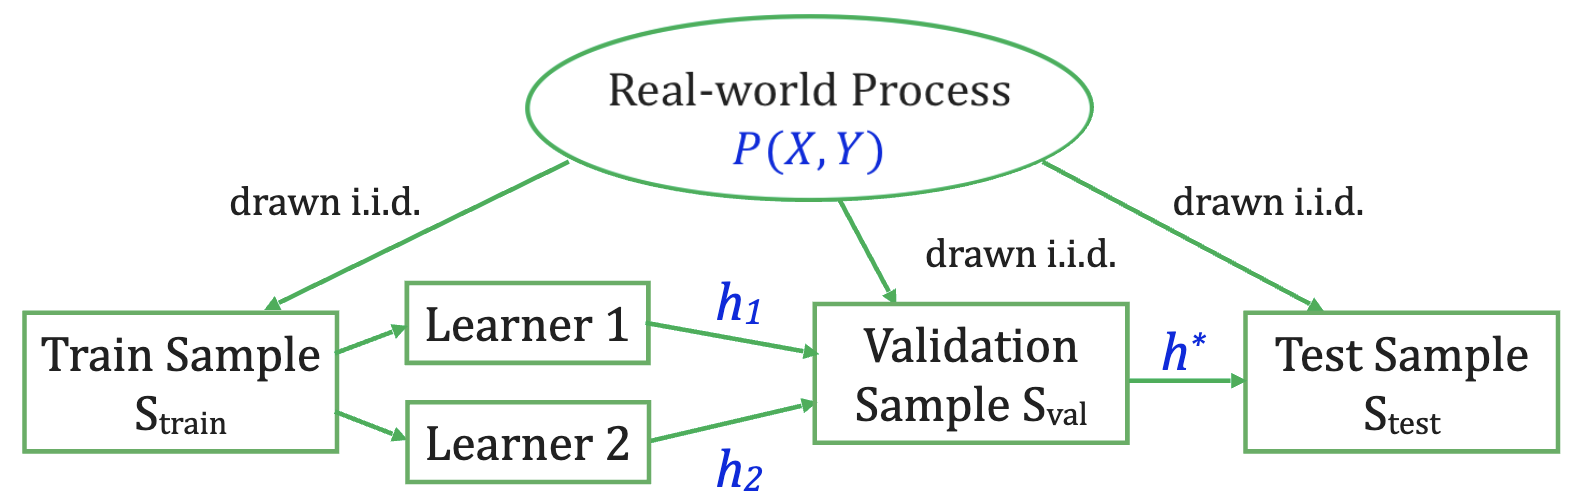
\includegraphics[width=0.8\textwidth]{Images/validation_sample.png}
    % \caption{Caption}
    % \label{fig:my_label}
\end{figure*}
\begin{itemize}
    \item \textbf{Training:} Run learning algorithm $l$ times (e.g. different parameters).
    \item \textbf{Validation Error:} Errors $err_{S_{val}}(h_i)$ are estimates of $err_{p}(h_i)$ for each $h_i$.
    \item \textbf{Selection:} Use $h^*$ with $\min\, err_{S_{val}}(\hat{h}_i)$ for prediction on test examples.
\end{itemize}

\paragraph{Two Nested Learning Algorithms}
\begin{itemize}
    \item \textbf{Primary Learning Algorithm on $S_{train}$}
    \begin{itemize}
        \item For each variant $A_1 \ldots A_l$ of learning algorithm, $h_i = A_i(S_{train})$
        \item Example: Decision Tree (DT) that stops at $i$ nodes.
    \end{itemize}
    \item \textbf{Secondary Learning Algorithm on $S_{val}$}
    \begin{itemize}
        \item Hypothesis space: $H' = \{h_1, \ldots, h_l\}$
        \item Learning Algorithm: $h^* = \arg\min\limits_{h \in H'} \left[ err_{S_{val}}(h) \right]$
    \end{itemize}
\end{itemize}

\paragraph{Typical ML Experiment}
\begin{itemize}
    \item Collect data $S = \left\{ \left( \vec{x}_1, y_1 \right), \ldots, \left( \vec{x}_m, y_m \right) \right\}$
    \item Split randomly into $S_{\text{train}}$, $S_{\text{val}}$, $S_{\text{test}}$
    \item REPEAT
    \begin{itemize}
        \item Train on $S_{\text{train}}$
        \item Validate on $S_{\text{val}}$
    \end{itemize}
    \item UNTIL we think we have a good rule $h$.
    \item Test $h$ on $S_{\text{test}}$ to evaluate its accuracy/error.
\end{itemize}

\subsection{Cross-Validation}
k-fold Cross-Validation:
\begin{itemize}
    \item \textbf{Given:}
    \begin{itemize}
        \item Training examples $S$
        \item Learning algorithm $A_p$ with parameter $p$ (model architectures or hyperparameters)
    \end{itemize}
    \item \textbf{Compute:}
    \begin{itemize}
        \item Randomly partition $S$ into $k$ equally sized subsets $S_1, \ldots, S_k$
        \item For each value of $p$:
        \begin{itemize}
            \item For $i$ from $1$ to $k$:
            \begin{itemize}
                \item Train $A_p$ on $S \setminus S_i$ and get $h_i$
                \item Apply $h_i$ to $S_i$ and compute $err_{S_i}(h_i)$
            \end{itemize}
            \item Compute cross-validation error:
            \[
                err_{CV}(A_p) = \frac{1}{k} \sum_i err_{S_i}(h_i)
            \]
        \end{itemize}
    \end{itemize}
    \item \textbf{Selection:}
    \begin{itemize}
        \item Pick parameter $p^*$ that minimizes $err_{CV}(A_p)$
        \item Train $A_{p^*}(S)$ on full sample $S$ to get final $h$
    \end{itemize}
\end{itemize}

\subsection{Generalization Error of Hypothesis}

\begin{itemize}
    \item \textbf{Given}
    \begin{itemize}
        \item Samples $S_{\text{train}}$ and $S_{\text{test}}$ of labeled instances
        \item Learning Algorithm $A$
    \end{itemize}
    \item \textbf{Setup}
    \begin{itemize}
        \item Train learning algorithm $A$ on $S_{\text{train}}$, result is $h$
        \item Apply $h$ to $S_{\text{test}}$ and compare predictions against true labels
    \end{itemize}
    \item \textbf{Test}
    \begin{itemize}
        \item Error on test sample $err_{S_{\text{test}}}(h)$ is estimate of true error $err_{p}(h)$
        \item Compute confidence interval
    \end{itemize}
\end{itemize}

\subsection{Significance Testing with the Binomial Distribution}

\begin{itemize}
    \item \textbf{Goal:} Assess whether the observed error rate of a hypothesis $h$ on a test set provides statistically significant evidence that the true error rate $err_P(h)$ is below (or above) a certain threshold.
    \item \textbf{Null Hypothesis:} Assume $err_P(h) \geq \epsilon$ for some threshold $\epsilon$.
    \item \textbf{Test Statistic:} Let $m$ be the number of test examples, and $k$ the number of observed errors. Under the null hypothesis, the number of errors $X$ follows a Binomial distribution: $X \sim \text{Binomial}(m, \epsilon)$.
    \item \textbf{p-value:} Compute the probability of observing $k$ or fewer errors under the null hypothesis:
    \[
        p\text{-value} = P(X \leq k \mid p = \epsilon, m)
    \]
    \item \textbf{Decision:} If the $p$-value is less than the significance level (e.g., $0.05$ for $95\%$ confidence), reject the null hypothesis and conclude that there is significant evidence that $err_P(h) < \epsilon$.
    \item \textbf{Interpretation:} This test quantifies how likely it is to observe the empirical error rate (or lower) if the true error rate were at least $\epsilon$.
\end{itemize}

\subsection{Normal Confidence Intervals}

\begin{itemize}
    \item \textbf{Rule of thumb:} When $mp(1-p) \geq 5$, the binomial distribution can be approximated by a normal distribution $N(\mu, \sigma^2)$ with $\mu = mp$ and $\sigma^2 = mp(1-p)$.
    \item \textbf{Normal confidence interval (95\% confidence):}
    \[
        err_P(h) \in \left[ err_S(h) - 1.96 \sqrt{\frac{p(1-p)}{m}},\; err_S(h) + 1.96 \sqrt{\frac{p(1-p)}{m}} \right]
    \]
    \item With approximation $p \approx err_S(h) \; \rightarrow$ Called ``Standard Error'' confidence intervals.
\end{itemize}

\subsection{Hoeffding Bound for Generalization Error}

\begin{itemize}
    \item \textbf{Hoeffding Bound:} For any loss function that takes values in $[0,1]$ and any hypothesis $h$, with probability at least $1 - \delta$ (where $1-\delta$ is called the \textbf{confidence level}), over the random choice of test samples $S$ of size $m$, the following holds:
    \[
        err_P(h) \in \left[ err_S(h) - \sqrt{\frac{-0.5 \ln(\delta/2)}{m}},\; err_S(h) + \sqrt{\frac{-0.5 \ln(\delta/2)}{m}} \right]
    \]
    \item This means that, with probability at least $1-\delta$, the true error $err_P(h)$ lies within the interval centered at the empirical error $err_S(h)$, with a margin that decreases as the number of test samples $m$ increases.
    \item The parameter $1-\delta$ is the probability that the interval contains the true error. For example, if $\delta = 0.05$, then $1-\delta = 0.95$ corresponds to a $95\%$ confidence interval.
\end{itemize}

\subsection{McNemar's Test}

\begin{itemize}
    \item \textbf{Given:}
    \begin{itemize}
        \item Two hypotheses $h_1$ and $h_2$
        \item Test set $S_{test}$ with $m$ examples
    \end{itemize}
    \item \textbf{Null Hypothesis:} $err_P(h_1) = err_P(h_2)$
    \begin{itemize}
        \item Implies that $err_S(h_1)$ and $err_S(h_2)$ come from binomial distributions with the same $p$
        \item Implies that the number of wins $w$ (where $h_1$ is correct and $h_2$ is not) and losses $l$ (where $h_2$ is correct and $h_1$ is not) follow:
        \[
            W \sim \text{Binomial}(p=0.5,\, n=w+l)
        \]
    \end{itemize}
    \item \textbf{Test:}
    \begin{itemize}
        \item Count wins $w$ and losses $l$ on $S_{test}$
        \item Reject the null hypothesis with $95\%$ confidence if:
        \[
            P(W \leq w \mid p=0.5,\, n=w+l) < 0.025
        \]
        or
        \[
            P(W \geq w \mid p=0.5,\, n=w+l) < 0.025
        \]
        \item \textbf{Why 0.025 instead of 0.05?} \\
        The total significance level is $0.05$ for a $95\%$ confidence test, but since McNemar's test is two-sided (we care if either $h_1$ is significantly better than $h_2$ or vice versa), we split the significance level equally between both tails of the distribution: $0.025$ for each tail.
    \end{itemize}
\end{itemize}

\section{Linear Classifiers}
\textbf{Date:} \underline{Sep 11, 2025}

\subsection{Vectors and Hyperplanes}
\paragraph{Euclidean Embeddings}
Data are represented as $d$ dimensional vectors in $\mathbb{R}^d$. The choice of representation is part of "inductive bias".

\paragraph{Euclidean Norm}
The Euclidean norm of a vector $x \in \mathbb{R}^d$ is defined as:
\[||\vec{x}|| = \sqrt{\sum_{i=1}^{d} x_i^2}\]

\paragraph{Dot Product}
The dot product of two vectors $\vec{x}, \vec{y} \in \mathbb{R}^d$ is defined as:
\[
\langle \vec{x}, \vec{y} \rangle = \sum_{i=1}^{d} x_i y_i
\]
Alternative notation: $\vec{x} \cdot \vec{y}$ or $\vec{x}^T \vec{y}$.

\paragraph{Angle \& Projection}
$\vec{w} \cdot \vec{x} = ||\vec{w}|| ||\vec{x}|| \cos(\theta)$, where $\theta$ is the angle between $\vec{w}$ and $\vec{x}$, and $\frac{\vec{w} \cdot \vec{x}}{||\vec{w}||}$ is the signed length of the projection of $\vec{x}$ onto $\vec{w}$.

\begin{figure}[h]
    \centering
    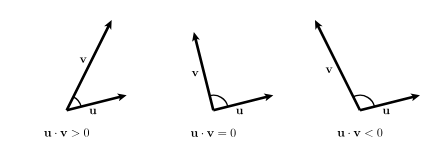
\includegraphics[width=0.5\textwidth]{Images/dot_product.png}
\end{figure}

\paragraph{Hyperplanes}
In $d$-dimensional space, a \textbf{hyperplane} is defined by a vector $\vec{w} \in \mathbb{R}^d$ and a scalar $b \in \mathbb{R}$:
\[
\left\{ \vec{x} \in \mathbb{R}^d \mid \vec{w} \cdot \vec{x} + b = 0 \right\}
\]

\textbf{Geometric interpretation:}
\begin{itemize}
    \item The hyperplane is orthogonal to $\vec{w}$.
    \item The distance to the origin (along $\vec{w}$) is $-\frac{b}{||\vec{w}||}$.
    \item All points on the hyperplane satisfy $\vec{w} \cdot \vec{x} = -b$.
\end{itemize}

\subsection{Linear Classifiers}

For a vector $\vec{w} \in \mathbb{R}^d$ and $b \in \mathbb{R}$, the hypothesis $h_{\vec{w},b} : \mathbb{R}^d \rightarrow \{-1, +1\}$ is called a $d$ dimensional linear classifier and defined as
\[
h_{\vec{w},b}(\vec{x}) = \mathrm{sign}(\vec{w} \cdot \vec{x} + b) =
\begin{cases}
+1 & \vec{w} \cdot \vec{x} + b > 0 \\
-1 & \vec{w} \cdot \vec{x} + b \leq 0
\end{cases}
\]

Also called linear predictor or halfspace.

\paragraph{Decision Boundaries in Different Dimensions}
\begin{itemize}
    \item \textbf{One dimension:} $h_{w,b}(x) = \mathrm{sign}(wx + b)$
    \begin{itemize}
        \item Decision boundary: a point (1d hyperplane) at $x = -\frac{b}{w}$
    \end{itemize}
    \item \textbf{Two dimensions:} $h_{\vec{w},b}(\vec{x}) = \mathrm{sign}(\vec{w} \cdot \vec{x} + b)$
    \begin{itemize}
        \item Decision boundary: a line (2d hyperplane) defined by $\vec{w} \cdot \vec{x} + b = 0$
    \end{itemize}
    \item \textbf{$d$ dimensions:} $\mathrm{sign}(\vec{w} \cdot \vec{x} + b)$
    \begin{itemize}
        \item Decision boundary: a hyperplane $\vec{w} \cdot \vec{x} + b = 0$
    \end{itemize}
\end{itemize}

\paragraph{Homogenous Linear Classifiers}

A classifier is \textbf{homogenous} if $b = 0$ (otherwise non-homogenous).

\textbf{Fact:} Any $d$ dimensional learning problem for linear classifiers has a \textbf{homogenous} form in $d+1$ dimensions.

\begin{center}
\begin{tabular}{|p{0.45\textwidth}|p{0.45\textwidth}|}
\hline
\textbf{Non-homogenous:} &
\textbf{Homogenous:} \\
\hline
$HS^d = \{ h_{\vec{w},b} \mid \vec{w} \in \mathbb{R}^d, b \in \mathbb{R} \}$

\begin{itemize}
    \item $\vec{x}$
    \item $\vec{w}, b$
    \item $\vec{w} \cdot \vec{x} + b$
\end{itemize}
&
$HS^{d+1}_{homog} = \{ h_{\vec{w},b} \mid \vec{w} \in \mathbb{R}^{d+1} \}$

\begin{itemize}
    \item $\vec{x}' = (\vec{x}, 1)$
    \item $\vec{w}' = (\vec{w}, b)$
    \item $\vec{w}' \cdot \vec{x}' = \vec{w} \cdot \vec{x} + b$
\end{itemize}
\\
\hline
\end{tabular}
\end{center}

Without loss of generality, we will now focus on \textbf{homogenous linear classifiers} with $||w_i|| = 1$.


\paragraph{Consistent Linear Classifiers}

\begin{itemize}
    \item Data set of labelled instances $\mathcal{S} = \{ (\vec{x}_1, y_1), (\vec{x}_2, y_2), \ldots, (\vec{x}_m, y_m) \}$.
    \item Linear classifier $h_{\vec{w}}$ is \textbf{consistent} with $\mathcal{S}$ if for all $(\vec{x}_i, y_i) \in \mathcal{S}$:
    \begin{itemize}
        \item $\vec{w} \cdot \vec{x}_i > 0$ if $y_i = 1$
        \item $\vec{w} \cdot \vec{x}_i \leq 0$ if $y_i = -1$
    \end{itemize}
    \item Data set $\mathcal{S}$ is \textbf{linearly separable} (zero training error) if there is a linear classifier $h_{\vec{w}}$ that is consistent with it.
\end{itemize}

\paragraph{Margin}
A data set $\mathcal{S}$ is linearly separable with a \textbf{(geometric) margin} $\gamma$ if:
\begin{itemize}
    \item There is a linear classifier $h_{\vec{w}}$ that is consistent with $\mathcal{S}$.
    \item The distance of any instance in $\mathcal{S}$ to the decision boundary of $h_{\vec{w}}$ is at least $\gamma$.
\end{itemize}

\textbf{Mathematical definition:} There is $\vec{w}$ such that $||\vec{w}|| = 1$ and for all data points $(\vec{x}_i, y_i) \in \mathcal{S}$:
\[
\begin{cases}
    \vec{w} \cdot \vec{x}_i \geq \gamma & \text{if } y_i = 1 \\
    \vec{w} \cdot \vec{x}_i \leq -\gamma & \text{if } y_i = -1
\end{cases}
\qquad \Longleftrightarrow \qquad
y_i (\vec{w} \cdot \vec{x}_i) \geq \gamma
\]

\textbf{Larger margin} $\implies$ \textbf{Easier to find consistent linear classifier}.

\subsection{Perceptron Algorithm}

\begin{algobox}
    \textbf{The Perceptron Algorithm (homogeneous \& batch)}

    \begin{itemize}
        \item \textbf{Input:} training data $\mathcal{S} = \{ (\vec{x}_1, y_1), \ldots, (\vec{x}_m, y_m) \}$
        \item \textbf{Initialize} $\vec{w}^{(0)} = (0, \ldots, 0)$ and $t = 0$
        \item \textbf{While} there is $i \in [m]$ such that $y_i (\vec{w}^{(t)} \cdot \vec{x}_i) \leq 0$:
        \begin{itemize}
            \item $\vec{w}^{(t+1)} = \vec{w}^{(t)} + y_i \vec{x}_i$
            \item $t \leftarrow t + 1$
        \end{itemize}
        \item \textbf{End While}
        \item \textbf{Output} $\vec{w}^{(t)}$
    \end{itemize}
\end{algobox}
Good Practice: Initialize $\vec{w}^{(0)}$ randomly. Shuffle $\mathcal{S}$ and check data one-by-one for update condition. Iterate until no updates are needed or maximum iterations are reached.

\section{Perceptron}
\textbf{Date:} \underline{Sep 16, 2025}

\begin{itemize}
    \item \textbf{Theorem:} Given a dataset $S = \{(\vec{x}_1, y_1), \ldots, (\vec{x}_m, y_m)\}$ and a radius $R$ such that $\|\vec{x}_i\| \leq R$ for all $i \in [m]$. If $S$ is linearly separable with (geometric) \textbf{margin} $\gamma$, then Perceptron makes at most $R^2/\gamma^2$ updates before finding a consistent linear classifier.
    \item This upper bound holds even if
    \begin{itemize}
        \item We scale every instance in the training set
        \item We shuffle the training set
        \item We don't know the value of $\gamma$
    \end{itemize}
    \item Actual number of updates can vary, but we know it cannot be more than $R^2/\gamma^2$
\end{itemize}



\section{Support Vector Machines}
\textbf{Date:} \underline{Sep 18, 2025}

\begin{itemize}
    \item \textbf{Assumption:} Training examples are linearly separable.
    \item \textbf{Optimal Hyperplane:} The separating hyperplane that maximizes the distance to the closest training examples.
\end{itemize}

\subsection{Margin of a Linear Classifier}

\textbf{Definition:} For a linear classifier $h_{w,b}$, the (functional) margin $\gamma_i$ of an example $(x_i, y_i)$ with $x \in \mathbb{R}^N$ and $y \in \{-1, +1\}$ is
\[
\gamma_i = y_i \left( \vec{w} \cdot \vec{x}_i + b \right)
\]

\textbf{Definition:} The margin is called \textbf{geometric margin}, if $\|\vec{w}\| = 1$. For general $\vec{w}$, the term functional margin is used to indicate that the norm of $\vec{w}$ is not necessarily 1.

\textbf{Definition:} The (hard) margin of a linear classifier $h_{w,b}$ on sample $S$ is
\[
\gamma = \min_{(x_i, y_i) \in S} y_i \left( \vec{w} \cdot \vec{x}_i + b \right)
\]

\subsection{Computing Optimal Hyperplanes}

\begin{itemize}
    \item \textbf{Requirement:} Zero training error.
    \[
        \forall (\vec{x}_i, y_i) \in S: \quad y_i \left( \vec{w} \cdot \vec{x}_i + b \right) > 0
    \]
    \item \textbf{Additional Requirement:} Maximize the distance to the closest training examples.
    \[
        \max_{\vec{w}, b, \gamma} \gamma \quad \text{s.t.} \quad \gamma = \min_{(\vec{x}_i, y_i) \in S} \left| \frac{1}{\|\vec{w}\|} \left( \vec{w} \cdot \vec{x}_i + b \right) \right|
    \]
    \item \textbf{Combine:}
    \[
        \max_{\vec{w}, b, \gamma} \gamma \quad \text{s.t.} \quad \gamma = \min_{(\vec{x}_i, y_i) \in S} \left[ \frac{y_i}{\|\vec{w}\|} \left( \vec{w} \cdot \vec{x}_i + b \right) \right]
    \]
\end{itemize}

We can rewrite the minimization as a set of constraints:
\[
\max_{\vec{w}, b, \gamma} \gamma \quad \text{s.t.} \quad \forall (\vec{x}_i, y_i) \in S: \frac{y_i}{\|\vec{w}\|} \left( \vec{w} \cdot \vec{x}_i + b \right) \geq \gamma
\]

This problem is invariant to scaling of $\vec{w}$ and $b$. We can fix the scale by setting $\|\vec{w}\| = 1/\gamma$:
\[
\max_{\vec{w}, b} \frac{1}{\|\vec{w}\|} \quad \text{s.t.} \quad \forall (\vec{x}_i, y_i) \in S: y_i \left( \vec{w} \cdot \vec{x}_i + b \right) \geq 1
\]

This is equivalent to minimizing $\|\vec{w}\|$:
\[
\min_{\vec{w}, b} \|\vec{w}\| \quad \text{s.t.} \quad \forall (\vec{x}_i, y_i) \in S: y_i \left( \vec{w} \cdot \vec{x}_i + b \right) \geq 1
\]

For mathematical convenience, we minimize $\frac{1}{2} \vec{w} \cdot \vec{w}$:
\[
\min_{\vec{w}, b} \frac{1}{2} \vec{w} \cdot \vec{w} \quad \text{s.t.} \quad \forall (\vec{x}_i, y_i) \in S: y_i \left( \vec{w} \cdot \vec{x}_i + b \right) \geq 1
\]

This is the standard form of the hard-margin SVM optimization problem.

\subsection{Hard Margin SVM}

\begin{itemize}
    \item \textbf{Goal:} Find the separating hyperplane with the largest distance (margin) to the closest training examples.
    \item \textbf{Optimization Problem:}
    \[
        \min_{\vec{w}, b} \frac{1}{2} \vec{w} \cdot \vec{w} \quad \text{s.t.} \quad y_i(\vec{w} \cdot \vec{x}_i + b) \geq 1 \quad \forall i
    \]
    \item \textbf{Support Vectors:} Training examples that lie exactly on the margin, i.e.,
    \[
        y_i(\vec{w} \cdot \vec{x}_i + b) = 1
    \]
    \item The margin $\gamma$ is the distance from the hyperplane to the closest points (support vectors).
    \item Limitations: For some training data, there is no separating hyperplane. Complete separation (i.e. zero training error) can lead to suboptimal prediction error.
\end{itemize}

\subsection{Soft Margin SVM}
\begin{itemize}
    \item \textbf{Idea:} Maximize margin and minimize training error. Allows some misclassification by introducing slack variables $\xi_i$.
    \item \textbf{Optimization Problem (Primal):}
    \[
        \min_{\vec{w}, b, \vec{\xi}} \frac{1}{2} \vec{w} \cdot \vec{w} + C \sum_{i=1}^n \xi_i
    \]
    \[
        \text{s.t.} \quad y_i(\vec{w} \cdot \vec{x}_i + b) \geq 1 - \xi_i, \quad \xi_i \geq 0 \quad \forall i
    \]
    \item \textbf{Slack variable} $\xi_i$ measures how much $(x_i, y_i)$ fails to achieve the margin.
    \begin{itemize}
        \item \textbf{Idea:} Slack variables $\xi_i$ capture training error.
        \item For any training example $(\vec{x}_i, y_i)$:
        \begin{itemize}
            \item $\xi_i \geq 1 \iff y_i(\vec{w} \cdot \vec{x}_i + b) \leq 0$ (error)
            \item $0 < \xi_i < 1 \iff 0 < y_i(\vec{w} \cdot \vec{x}_i + b) < 1$ (correct, but within margin)
            \item $\xi_i = 0 \iff y_i(\vec{w} \cdot \vec{x}_i + b) \geq 1$ (correct)
        \end{itemize}
        \item The sum $\sum_i \xi_i$ is an upper bound on the number of training errors.
        \item $C$ controls the trade-off between margin size and training error.
    \end{itemize}
    \item Examples with margin less than or equal to 1 are support vectors.
\end{itemize}

\section{Kernels and Duality}
\textbf{Date:} \underline{Sep 23, 2025}

\paragraph{Non-linear Problems}
Some tasks have non-linear structure, and no hyperplane is sufficiently accurate.

For those problems, we can extend the feature space. For example, for quadratic features, we can have:
\begin{itemize}
    \item \textbf{Input Space:} $\vec{x} = (x_1, x_2)$ \hspace{1cm} (2 attributes)
    \item \textbf{Feature Space:} $\Phi(\vec{x}) = (x_1^2, x_2^2, x_1, x_2, x_1 x_2, 1)$ \hspace{1cm} (6 attributes)
\end{itemize}

\paragraph{SVM with Feature Map}
Support Vector Machines (SVMs) can use a feature map $\Phi(\vec{x})$ to transform the input into a higher-dimensional space, making non-linear problems linearly separable.

\begin{itemize}
    \item \textbf{Training:} SVMs solve the following optimization problem:
    \begin{align*}
        \text{minimize:} \quad & P(\vec{w}, b, \vec{\xi}) = \frac{1}{2} \vec{w} \cdot \vec{w} + C \sum_{i=1}^n \xi_i \\
        \text{subject to:} \quad & y_i [\vec{w} \cdot \Phi(\vec{x}_i) + b] \geq 1 - \xi_i \quad \forall i \\
        & \xi_i > 0 \quad \forall i
    \end{align*}
    \item \textbf{Classification:} The decision function is:
    \[
        h(\vec{x}) = \text{sign} \left[ \vec{w}^* \cdot \Phi(\vec{x}) + b \right]
    \]
\end{itemize}

\textbf{Problems:}
\begin{itemize}
    \item \textbf{Computational Challenge:} Mapping to high-dimensional feature spaces can be computationally expensive.
    \item \textbf{Overfitting:} Using many features increases the risk of overfitting, so regularization and careful kernel choice are important.
\end{itemize}

\subsection{Dual Perceptron}

\paragraph{(Batch) Perceptron Algorithm}
\begin{itemize}
    \item Initialize $\vec{\alpha} = \vec{0}$ (the dual variables)
    \item Repeat for $E$ epochs:
    \begin{itemize}
        \item For $i = 1$ to $m$:
        \begin{itemize}
            \item If $y_i \left( \sum_{j=1}^m \alpha_j y_j (\vec{x}_j \cdot \vec{x}_i) \right) \leq 0$ then $\alpha_i = \alpha_i + 1$
        \end{itemize}
    \end{itemize}
    \item The prediction for a new $\vec{x}$ is:
    \[
        h(\vec{x}) = \text{sign} \left( \sum_{j=1}^m \alpha_j y_j (\vec{x}_j \cdot \vec{x}) \right)
    \]
\end{itemize}

\[
    \vec{w} \cdot \vec{x}_i = 
    \left( \sum_{j=1}^m \alpha_j y_j \vec{x}_j \right) \cdot \vec{x}_i = 
    \sum_{j=1}^m \alpha_j y_j (\vec{x}_j \cdot \vec{x}_i)
\]

Instead of tracking the weight, we track the number of updates made by each training example.
The hyperplane output by the Perceptron can always be expressed as a linear combination of the training data.

\paragraph{Primal vs. Dual Representation}

\begin{itemize}
    \item Primal Representation:
    \begin{itemize}
        \item Weight vector $\vec{w} \in \mathbb{R}^d$
        \item Threshold $b \in \mathbb{R}$
    \end{itemize}
    \item Dual Representation:
    \begin{itemize}
        \item Training data $(\vec{x}_1, y_1), \ldots, (\vec{x}_m, y_m)$
        \item Vector of dual variables $\vec{\alpha}$
        \item Threshold $b \in \mathbb{R}$
    \end{itemize}
\end{itemize}

\paragraph{What is Duality good for?}

\begin{enumerate}
    \item Dual variables give insight into the data.
    \item If dimensionality $d$ of $\vec{x}$ is large, working in the dual representation can be more efficient if $\vec{x}_i \cdot \vec{x}_j$ is efficient.
    \item Duality lets us prove theorems about the generalization error of the classifier.
\end{enumerate}

\subsection{Dual SVM}

\begin{itemize}
    \item \textbf{Primal Optimization Problem:}
    \begin{align*}
        \text{minimize:} \quad & P(\vec{w}, b, \vec{\xi}) = \frac{1}{2} \vec{w} \cdot \vec{w} + C \sum_{i=1}^n \xi_i \\
        \text{subject to:} \quad & y_i [\vec{w} \cdot \vec{x}_i + b] \geq 1 - \xi_i \quad \forall i \\
        & \xi_i \geq 0 \quad \forall i
    \end{align*}

    \item \textbf{Dual Optimization Problem:}
    \begin{align*}
        \text{maximize:} \quad & D(\vec{\alpha}) = \sum_{i=1}^n \alpha_i - \frac{1}{2} \sum_{i=1}^n \sum_{j=1}^n y_i y_j \alpha_i \alpha_j (\vec{x}_i \cdot \vec{x}_j) \\
        \text{subject to:} \quad & \sum_{i=1}^n y_i \alpha_i = 0 \\
        & 0 \leq \alpha_i \leq C \quad \forall i
    \end{align*}

    \item \textbf{Theorem:} If $(\vec{w}^*, b^*, \vec{\xi}^*)$ is the solution of the Primal and $\vec{\alpha}^*$ is the solution of the Dual, then
    \[
        \vec{w}^* = \sum_{i=1}^m \alpha_i^* y_i \vec{x}_i
        \qquad \text{and} \qquad
        P(\vec{w}^*, b^*, \vec{\xi}^*) = D(\vec{\alpha}^*)
    \]
\end{itemize}

Dual variable $\alpha_i$ is proportional to force on data point.
More formally, Dual variable $\alpha_i^*$ indicates the ``influence'' of training example $(\vec{x}_i, y_i)$.

\begin{itemize}
    \item $\vec{w}^* = \sum_{i=1}^m \alpha_i^* y_i \vec{x}_i$
    \item \textbf{Definition:} $(\vec{x}_i, y_i)$ is a \textit{support vector} (SV) if and only if $\alpha_i^* > 0$.
    \item If $\xi_i^* > 0$, then $\alpha_i^* = C$.
    \item If $0 \leq \alpha_i^* < C$, then $\xi_i^* = 0$.
    \item If $0 < \alpha_i^* < C$, then $y_i \left( \vec{x}_i \cdot \vec{w}^* + b^* \right) \text{(functional margin)} = 1$.
\end{itemize}

\paragraph{Leave-One-Out Error and Support Vectors}

Leave-one-out (LOO) cross validation is a good estimate of the generalization error for large $n$:
\[
    err_{loo}(A(S)) \approx err_P(A(S))
\]

\textbf{Theorem [Vapnik]:} For any SVM,
\[
    err_{loo}(SVM(S)) \leq \frac{1}{m} \#SV
\]
where $\#SV$ is the number of support vectors.

\textbf{Theorem [Vapnik]:} For a homogeneous hard-margin SVM,
\[
    err_{loo}(SVM(S)) \leq \frac{1}{m} \frac{R^2}{\gamma^2}
\]
where
\[
    R^2 = \max_{i \in [1..m]} \vec{x}_i \cdot \vec{x}_i
\]
and $\gamma$ is the margin on the training sample $S$.

\subsection{Non-Linear Rules through Kernels}

\paragraph{Kernel Trick}

Instead of explicitly mapping $\vec{x}$ to a high-dimensional feature space, we use a \textbf{kernel function} $K(\vec{x}, \vec{z})$ that computes the inner product in the feature space:
\[
    K(\vec{x}, \vec{z}) = \Phi(\vec{x}) \cdot \Phi(\vec{z})
\]
This allows us to run algorithms that depend only on dot products without ever computing $\Phi(\vec{x})$ directly.

\paragraph{Polynomial Kernel Example}

For $\vec{x} = (x_1, x_2)$, the degree-2 polynomial kernel is:
\[
    K(\vec{x}, \vec{z}) = (\vec{x} \cdot \vec{z} + 1)^2
\]
This corresponds to the feature map:
\[
    \Phi(\vec{x}) = (x_1^2,\, x_2^2,\, \sqrt{2}x_1,\, \sqrt{2}x_2,\, \sqrt{2}x_1x_2,\, 1)^\top
\]
so that
\[
    K(\vec{x}, \vec{z}) = \Phi(\vec{x}) \cdot \Phi(\vec{z})
\]

\paragraph{SVM with Kernel}

\begin{itemize}
    \item \textbf{Dual Optimization with Kernel:}
    \begin{align*}
        \text{maximize:} \quad & D(\vec{\alpha}) = \sum_{i=1}^n \alpha_i - \frac{1}{2} \sum_{i=1}^n \sum_{j=1}^n y_i y_j \alpha_i \alpha_j K(\vec{x}_i, \vec{x}_j) \\
        \text{subject to:} \quad & \sum_{i=1}^n y_i \alpha_i = 0 \\
        & 0 \leq \alpha_i \leq C \quad \forall i
    \end{align*}
    \item \textbf{Classification Rule:}
    \[
        h(\vec{x}) = \text{sign} \left( \sum_{i=1}^n \alpha_i y_i K(\vec{x}_i, \vec{x}) + b \right)
    \]
    \item \textbf{Common Kernels:}
    \begin{itemize}
        \item Linear: $K(\vec{a}, \vec{b}) = \vec{a} \cdot \vec{b}$
        \item Polynomial: $K(\vec{a}, \vec{b}) = (\vec{a} \cdot \vec{b} + 1)^k$
        \item Radial Basis Function (RBF): $K(\vec{a}, \vec{b}) = \exp\left(-\gamma \|\vec{a} - \vec{b}\|^2\right)$
        \item Sigmoid: $K(\vec{a}, \vec{b}) = \tanh(\gamma \vec{a} \cdot \vec{b} + c)$
    \end{itemize}
\end{itemize}

The kernel trick allows SVMs to efficiently learn non-linear decision boundaries by implicitly operating in high-dimensional feature spaces.

\subsection{Designing Kernels}

\paragraph{Definition:}
Let $X$ be a nonempty set. A function $K$ is a \textbf{valid} kernel in $X$ if for all $m$ and all $x_1, \ldots, x_m \in X$, it produces a Gram matrix
\[
    G_{ij} = K(x_i, x_j)
\]
that is symmetric
\[
    G = G^T
\]
and positive semi-definite
\[
    \forall \vec{\alpha} : \vec{\alpha}^T G \vec{\alpha} \geq 0
\]

Any inner product is a kernel. Most properties of inner products also hold for kernels.

\paragraph{How to Construct Kernels}

\paragraph{Theorem:}
Let $K_1$ and $K_2$ be valid kernels over $X \times X$, $\alpha \geq 0$, $0 \leq \lambda \leq 1$, $f$ a real-valued function on $X$, $\Phi: X \to \mathbb{R}^N$ with a kernel $K_3$ over $\mathbb{R}^N \times \mathbb{R}^N$, and $K$ a symmetric positive semi-definite matrix. Then the following functions are valid kernels:
\begin{align*}
    K(\vec{x}, \vec{z}) &= \lambda K_1(\vec{x}, \vec{z}) + (1 - \lambda) K_2(\vec{x}, \vec{z}) \\
    K(\vec{x}, \vec{z}) &= \alpha K_1(\vec{x}, \vec{z}) \\
    K(\vec{x}, \vec{z}) &= K_1(\vec{x}, \vec{z}) K_2(\vec{x}, \vec{z}) \\
    K(\vec{x}, \vec{z}) &= f(\vec{x}) f(\vec{z}) \\
    K(\vec{x}, \vec{z}) &= K_3(\Phi(\vec{x}), \Phi(\vec{z})) \\
    K(\vec{x}, \vec{z}) &= \vec{x}^T K \vec{z}
\end{align*}

These closure properties allow us to construct new valid kernels from existing ones.

\subsection{Properties of SVMs with Kernels}

\begin{itemize}
    \item \textbf{Expressiveness}
    \begin{itemize}
        \item SVMs with kernels can represent any boolean function (for appropriate choice of kernel).
        \item SVMs with kernels can represent any sufficiently ``smooth'' function to arbitrary accuracy (for appropriate choice of kernel).
    \end{itemize}
    \item \textbf{Computational}
    \begin{itemize}
        \item Objective function has no local optima (only one global optimum).
        \item Independent of dimensionality of feature space.
    \end{itemize}
    \item \textbf{Generalization Error}
    \begin{itemize}
        \item Low leave-one-out error if dual solution is sparse.
        \item Low leave-one-out error if $\frac{R^2}{\gamma^2}$ is small.
    \end{itemize}
    \item \textbf{Design decisions}
    \begin{itemize}
        \item Kernel type and parameters.
        \item Value of $C$.
    \end{itemize}
\end{itemize}

\section{Regularized Linear Models}
\textbf{Date:} \underline{Sep 25, 2025}

\subsection{ERM Learning}

\begin{itemize}
    \item \textbf{Examples:} KNN, decision trees, Perceptron, SVM.
    \item \textbf{Modelling Step:} Select a family of classification rules $\mathcal{H}$ to consider (hypothesis space, features).
    \item \textbf{Training Principle:}
    \begin{itemize}
        \item Given training sample $(\vec{x}_1, y_1), \ldots, (\vec{x}_n, y_n)$
        \item Find $h \in \mathcal{H}$ with lowest training error
        \item This is called \textit{Empirical Risk Minimization (ERM)}
    \end{itemize}
    \item \textbf{Argument:} Low training error leads to low prediction error, if overfitting is controlled (\textit{generalization}).
\end{itemize}

\subsection{Bayes Decision Rule (0/1 loss)}
\begin{itemize}
    \item \textbf{Assumption:} The decision setting is known: $P(X,Y) = P(Y\mid X)P(X)$.
    \item \textbf{Goal:} For a given instance $\vec{x}$, choose $\hat{y}$ to minimize prediction error under $0/1$ loss
    \[
      L_{0/1}(\hat{y},y)=\begin{cases}
      1,& \hat{y}\neq y\\
      0,& \hat{y}=y~.
      \end{cases}
    \]
    \item \textbf{Rule:} 
    \[
      h_{\text{Bayes}}(\vec{x})=\arg\max_{y\in\mathcal{Y}} P(Y=y\mid X=\vec{x}).
    \]
\end{itemize}

\subsection{Decision via Bayes Risk}
\begin{itemize}
    \item \textbf{Bayes Risk} (expected loss of classifier $h$ under distribution $P$ and loss $L$):
    \[
      \mathrm{Err}_{P}(h)=\mathbb{E}_{\vec{x},y\sim P(X,Y)}\!\!\big[L(h(\vec{x}),y)\big]
      =\mathbb{E}_{\vec{x}\sim P(X)}\big[\mathbb{E}_{y\sim P(Y\mid \vec{x})}[L(h(\vec{x}),y)]\big].
    \]
    \item \textbf{Bayes Decision Rule} minimizes the conditional risk:
    \[
      h_{\text{Bayes}}(\vec{x})=\arg\min_{\hat{y}\in\mathcal{Y}}
      \sum_{y\in\mathcal{Y}} L(\hat{y},y)\,P(Y=y\mid X=\vec{x}).
    \]
    \item \textbf{Minimal risk for $0/1$ loss:}
    \[
      \mathrm{Err}_{P}(h_{\text{Bayes}})
      =\mathbb{E}_{\vec{x}\sim P(X)}\!\left[1-\max_{y\in\mathcal{Y}} P(Y=y\mid X=\vec{x})\right].
    \]
\end{itemize}

\subsection{Learning Conditional Probabilities}
\begin{itemize}
    \item \textbf{Modeling:} Choose a parametric family $P(Y\mid X,\vec{w})$.
    \item \textbf{Training:} Given $(\vec{x}_i,y_i)_{i=1}^n$, find $\hat{\vec{w}}$ that best fits data:
    \begin{itemize}
        \item \textit{Maximum Likelihood (ML)} or \textit{Maximum a Posteriori (MAP)}.
    \end{itemize}
    \item \textbf{Classification:} Use Bayes rule with learned $P(Y\mid X,\hat{\vec{w}})$.
    \item \textbf{Argument:} If the learned conditional distribution is close to the true one, the induced decision rule is accurate.
\end{itemize}

\subsection{Logistic Regression Model (binary $y\in\{-1,+1\}$)}
\begin{itemize}
    \item \textbf{Likelihood:} $P(Y_i=y\mid \vec{x}_i,\vec{w})=\sigma(y\,\vec{w}\!\cdot\!\vec{x}_i)$,
    \qquad where $\displaystyle \sigma(z)=\frac{1}{1+e^{-z}}$.
    \item \textbf{Symmetry:} $1-\sigma(\vec{w}\!\cdot\!\vec{x})=\sigma(-\vec{w}\!\cdot\!\vec{x})$.
\end{itemize}

\subsection{Logistic Regression Training (Conditional MLE)}
\begin{itemize}
    \item \textbf{Objective:}
    \[
      \hat{\vec{w}}=\arg\max_{\vec{w}} \prod_{i=1}^n P(y_i\mid \vec{x}_i,\vec{w})
      \;=\; \arg\min_{\vec{w}} \sum_{i=1}^n \ln\!\big(1+e^{-y_i\,\vec{w}\cdot\vec{x}_i}\big).
    \]
    \item \textbf{Derivation Sketch:}
    \begin{enumerate}
        \item i.i.d.\ data $\Rightarrow$ factorized likelihood $\prod_i P(y_i\mid \vec{x}_i,\vec{w})$.
        \item Plug logistic form $P(y_i\mid \vec{x}_i,\vec{w})=\sigma(y_i\vec{w}\!\cdot\!\vec{x}_i)$.
        \item Apply $-\ln(\cdot)$ (monotone decreasing) and log-product $\ln\prod=\sum\ln$.
        \item Use $\sigma(z)=1/(1+e^{-z})$ to obtain logistic loss.
    \end{enumerate}
    \item \textbf{Prediction:} $h(\vec{x})=\operatorname{sign}(\hat{\vec{w}}\cdot \vec{x})$ (equivalently $\arg\max_y P(y\mid \vec{x},\hat{\vec{w}})$).
    \item \textbf{Issue (separable data):} If data are linearly separable, the MLE drives $\|\vec{w}\|\to\infty$ since $y_i\,\vec{w}\!\cdot\!\vec{x}_i>0$ can be increased without bound.
\end{itemize}

\subsection{Regularized Logistic Regression: Probabilistic View}
\begin{itemize}
    \item \textbf{Likelihood:} Same as above.
    \item \textbf{Prior on weights:} $\vec{w}\sim \mathcal{N}(\vec{0},\sigma^2 I)$, i.e.
    \[
      P(\vec{w})=\left(\frac{1}{\sigma\sqrt{2\pi}}\right)^{\!d}
      \exp\!\left(-\frac{\vec{w}\cdot\vec{w}}{2\sigma^2}\right).
    \]
    \item \textbf{MAP Training:}
    \[
      \hat{\vec{w}}
      =\arg\max_{\vec{w}} P(\vec{w})\prod_{i=1}^n P(y_i\mid \vec{x}_i,\vec{w})
      =\arg\min_{\vec{w}}
      \left\{\frac{\|\vec{w}\|_2^2}{2\sigma^2}+\sum_{i=1}^n \ln\!\big(1+e^{-y_i\,\vec{w}\cdot\vec{x}_i}\big)\right\}.
    \]
    \item \textbf{Equivalent scaled form (ignore positive constants):}
    \[
      \hat{\vec{w}}=\arg\min_{\vec{w}}
      \left\{\frac{1}{2}\|\vec{w}\|_2^2+\sigma^{2}\sum_{i=1}^n \ln\!\big(1+e^{-y_i\,\vec{w}\cdot\vec{x}_i}\big)\right\}.
    \]
    \item \textbf{Interpretation:} Gaussian prior $\Rightarrow$ $\ell_2$-regularization; controls $\|\vec{w}\|$ and prevents blow-up on separable data.
\end{itemize}

\subsection{Regularized Logistic Regression: Summary}
\begin{itemize}
    \item \textbf{Training Objective (ridge-regularized log-loss):}
    \[
      \hat{\vec{w}}=\arg\min_{\vec{w}} \;\frac{\lambda}{2}\|\vec{w}\|_2^2
      + \sum_{i=1}^n \ln\!\big(1+e^{-y_i\,\vec{w}\cdot\vec{x}_i}\big),
      \quad \text{with } \lambda=\frac{1}{\sigma^2}.
    \]
    \item \textbf{Prediction:} $h(\vec{x})=\arg\max_{y}P(y\mid \vec{x},\hat{\vec{w}})=\mathrm{sign}(\hat{\vec{w}}\cdot \vec{x})$.
\end{itemize}

\subsection{Linear Regression Model}
\begin{itemize}
    \item \textbf{Data:} $\mathcal{S}=\{(\vec{x}_1,y_1),\ldots,(\vec{x}_n,y_n)\}$ with $\vec{x}_i\in\mathbb{R}^d$ and $y_i\in\mathbb{R}$.
    \item \textbf{Likelihood model:} $Y_i\mid \vec{x}_i,\vec{w}\sim \mathcal{N}(\vec{w}\!\cdot\!\vec{x}_i,\eta^2)$, i.e.
    \[
      P(Y_i=y\mid \vec{x}_i,\vec{w})=\frac{1}{\eta\sqrt{2\pi}}
      \exp\!\left(-\frac{(\vec{w}\!\cdot\!\vec{x}_i-y)^2}{2\eta^2}\right).
    \]
\end{itemize}

\subsection{Linear Regression Training (Conditional MLE)}
\begin{itemize}
    \item \textbf{Objective:}
    \[
      \hat{\vec{w}}=\arg\max_{\vec{w}} \prod_{i=1}^n P(y_i\mid \vec{x}_i,\vec{w})
      \;=\; \arg\min_{\vec{w}} \sum_{i=1}^n \Big[-\ln P(y_i\mid \vec{x}_i,\vec{w})\Big].
    \]
    \item \textbf{Derivation:}
    \[
      \hat{\vec{w}}
      =\arg\min_{\vec{w}} \sum_{i=1}^n \left[-\ln\!\Big(\tfrac{1}{\eta\sqrt{2\pi}}\Big) 
      + \frac{(\vec{w}\!\cdot\!\vec{x}_i-y_i)^2}{2\eta^2}\right]
      =\arg\min_{\vec{w}} \frac{1}{2\eta^2}\sum_{i=1}^n(\vec{w}\!\cdot\!\vec{x}_i-y_i)^2.
    \]
    \item \textbf{Conclusion:} MLE $\Longleftrightarrow$ least-squares (ignoring positive constants).
    \item \textbf{Prediction:} $h(\vec{x})=\arg\max_y P(y\mid \vec{x},\hat{\vec{w}})=\hat{\vec{w}}\!\cdot\!\vec{x}$ (posterior mean for Gaussian).
\end{itemize}

\subsection{Ridge Regression (MAP for a Gaussian prior)}
\begin{itemize}
    \item \textbf{Likelihood:} same as linear regression:
    $P(Y_i\mid \vec{x}_i,\vec{w})=\mathcal{N}(\vec{w}\!\cdot\!\vec{x}_i,\eta^2)$.
    \item \textbf{Prior:} $\vec{w}\sim \mathcal{N}(\vec{0},\sigma^2 I)$ with
    \[
      P(\vec{w})=\left(\frac{1}{\sigma\sqrt{2\pi}}\right)^d
      \exp\!\left(-\frac{\vec{w}\!\cdot\!\vec{w}}{2\sigma^2}\right).
    \]
    \item \textbf{MAP training:}
    \[
      \hat{\vec{w}}=\arg\max_{\vec{w}} P(\vec{w})\prod_{i=1}^n P(y_i\mid \vec{x}_i,\vec{w})
      =\arg\min_{\vec{w}} \left\{\frac{\vec{w}\!\cdot\!\vec{w}}{2\sigma^2}
      +\frac{1}{2\eta^2}\sum_{i=1}^n(\vec{w}\!\cdot\!\vec{x}_i-y_i)^2\right\}.
    \]
    \item \textbf{Scaled form (drop positive constants):}
    \[
      \hat{\vec{w}}=\arg\min_{\vec{w}} \frac{1}{2}\|\vec{w}\|_2^2
      + C\sum_{i=1}^n(\vec{w}\!\cdot\!\vec{x}_i-y_i)^2,
      \qquad \text{where } C=\frac{\sigma^2}{2\eta^2}.
    \]
    \item \textbf{Prediction:} $h(\vec{x})=\hat{\vec{w}}\!\cdot\!\vec{x}$.
\end{itemize}

\subsection{Discriminative Training: A Unifying View}
\begin{itemize}
    \item \textbf{Template objective:}
    \[
      \min_{\vec{w}}\; R(\vec{w}) \;+\; C\sum_{i=1}^n L\!\big(\vec{w}\!\cdot\!\vec{x}_i,\,y_i\big).
    \]
    \item \textbf{Examples (classification):}
    \begin{itemize}
        \item \textit{Soft-margin SVM:} $R(\vec{w})=\tfrac{1}{2}\vec{w}\!\cdot\!\vec{w}$,\quad
        $L(\hat{y},y)=\max(0,1-y\hat{y})$.
        \item \textit{Perceptron:} $R(\vec{w})=0$,\quad $L(\hat{y},y)=\max(0,-y\hat{y})$.
        \item \textit{Reg.\ Logistic Regression:} $R(\vec{w})=\tfrac{1}{2}\vec{w}\!\cdot\!\vec{w}$,\quad
        $L(\hat{y},y)=\ln\!\big(1+e^{-y\hat{y}}\big)$.
    \end{itemize}
    \item \textbf{Examples (regression):}
    \begin{itemize}
        \item \textit{Linear Regression:} $R(\vec{w})=0$,\quad $L(\hat{y},y)=(y-\hat{y})^2$.
        \item \textit{Ridge Regression:} $R(\vec{w})=\tfrac{1}{2}\vec{w}\!\cdot\!\vec{w}$,\quad $L(\hat{y},y)=(y-\hat{y})^2$.
        \item \textit{Lasso:} $R(\vec{w})=\lambda\sum_{j=1}^d |w_j|$,\quad $L(\hat{y},y)=(y-\hat{y})^2$.
    \end{itemize}
\end{itemize}

\subsection{``45 ML Algorithms on 1 Slide'': Building Blocks}
\begin{itemize}
    \item \textbf{Common loss functions $L$:}
    \begin{itemize}
        \item Hinge: $\max(0,1-y\hat{y})$
        \item Logistic: $\ln\!\big(1+e^{-y\hat{y}}\big)$
        \item Exponential: $e^{-y\hat{y}}$
        \item Squared error: $(y-\hat{y})^2$
        \item Absolute error: $\lvert y-\hat{y}\rvert$
    \end{itemize}
    \item \textbf{Common regularizers $R$:}
    \begin{itemize}
        \item $\ell_2$: $\vec{w}\!\cdot\!\vec{w}$
        \item $\ell_1$: $\sum_{j=1}^d |w_j|$
        \item $\ell_0$: $\big|\{j: w_j\neq 0\}\big|$
    \end{itemize}
    \item \textbf{Beyond linear scores $\vec{w}\!\cdot\!\vec{x}$:}
    \begin{itemize}
        \item \textit{Kernels:} $\vec{w}\!\cdot\!\phi(\vec{x})$
        \item \textit{Deep networks:} $f(\vec{x};\vec{w})$
        \item \textit{Boosting:} $\sum_j \alpha_j\,\mathrm{Tree}_j(\vec{x})$
    \end{itemize}
\end{itemize}


\section{Optimization with Gradient Descent}
\textbf{Date:} \underline{Sep 30, 2025}

\section{Neural Networks}
\textbf{Date:} \underline{Oct 2, 2025}

\subsection{Multi-Layer Neural Networks}

\begin{center}
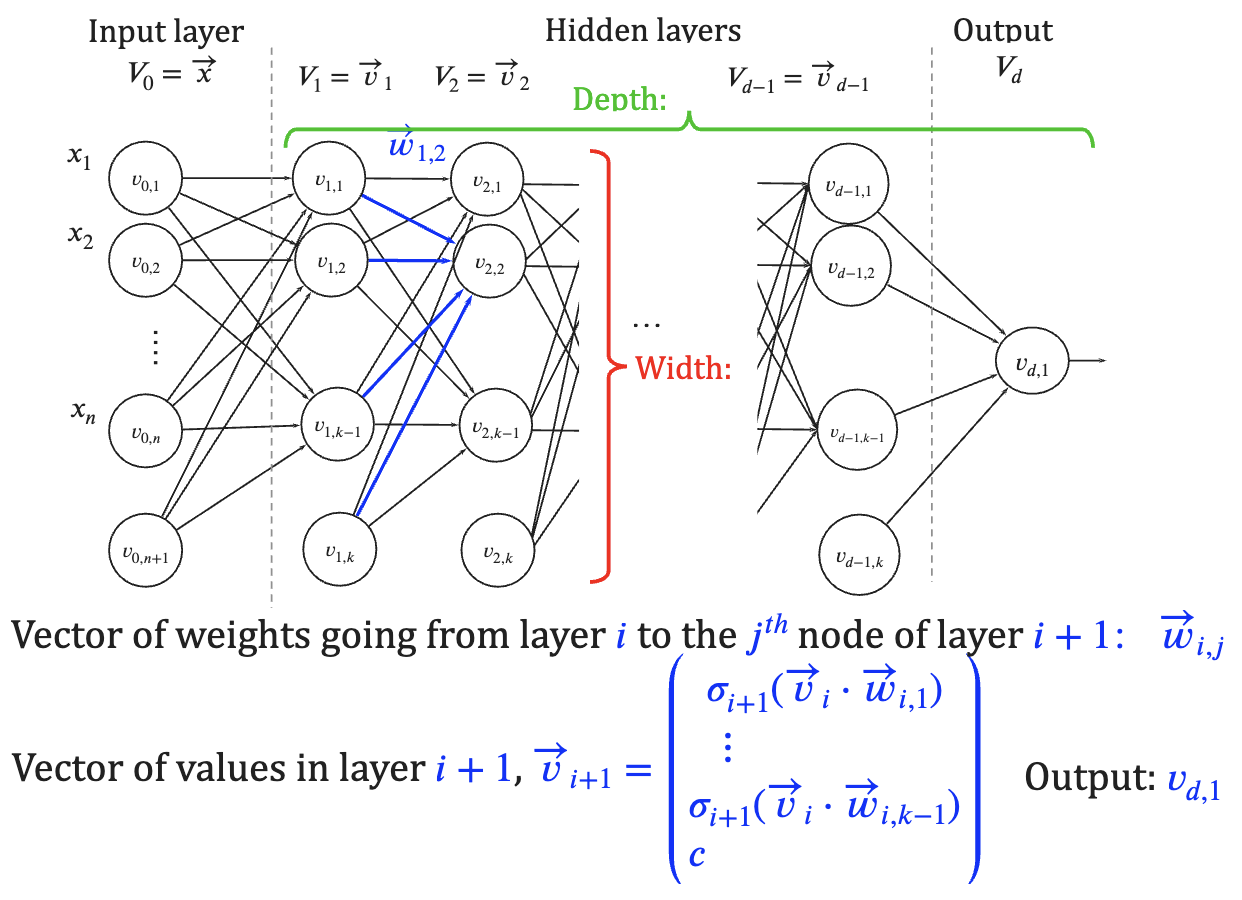
\includegraphics[width=0.6\textwidth]{Images/nn.png}
\end{center}

A multi-layer neural network (also called a feedforward neural network) consists of an input layer, one or more hidden layers, and an output layer. Each layer is made up of nodes (neurons), and each node in a layer is connected to every node in the next layer.
\begin{itemize}
    \item Let $\vec{v}_i$ be the vector of values in layer $i$.
    \item Let $\vec{w}_{i,j}$ be the vector of weights from layer $i$ to the $j$th node of layer $i+1$.
    \item The value at node $j$ in layer $i+1$ is computed as:
    \[
    v_{i+1, j} = \sigma_{i+1}(\vec{v}_i \cdot \vec{w}_{i,j})
    \]
    where $\sigma_{i+1}$ is the activation function for layer $i+1$.
\end{itemize}

\paragraph{Concise Matrix Formulation}

\begin{itemize}
    \item Let $W_i$ be the weight matrix for layer $i$, where each column $j$ is the weight vector $\vec{w}_{i,j}$.
    \item Layers are fully connected; any missing edge has weight $0$.
    \item The vector of activations for layer $i+1$ is:
    \[
    \vec{v}_{i+1} = \sigma_{i+1}(W_i^\top \vec{v}_i)
    \]
    where $\sigma_{i+1}$ is applied elementwise.
\end{itemize}


The output of a $d$-layer neural network can be written as a nested composition of linear transformations and activation functions:
\[
\sigma_d\left(W_{d-1}^\top \cdots\, \sigma_3\left(W_2^\top\, \sigma_2\left(W_1^\top\, \sigma_1\left(W_0^\top\, \vec{v}_0\right)\right)\right)\cdots\right)
\]
where each $\sigma_i$ is applied elementwise, and $W_i$ is the weight matrix for layer $i$.

\begin{algobox}
\textbf{Forward Propagation Algorithm:}

\textbf{Input:} Neural Network with weight matrices $W_0, W_1, \ldots, W_{d-1}$, activation functions $\sigma_1, \ldots, \sigma_d$ and instance $\vec{x}$

$\vec{v}_0 = \vec{x}$

\textbf{For} $\ell = 1, \ldots, d$
\begin{itemize}
    \item $\vec{s}_\ell = W_{\ell-1}^\top \vec{v}_{\ell-1}$
    \item $\vec{v}_\ell = \sigma_\ell(\vec{s}_\ell)$
\end{itemize}
\textbf{End For}

\textbf{Output} $\vec{v}_d$
\end{algobox}

\subsection{Non-linear Activation Functions}

Activation functions are applied to the nodes of a hidden layer in a neural network. They introduce non-linearity, allowing the network to learn complex patterns.

\begin{center}
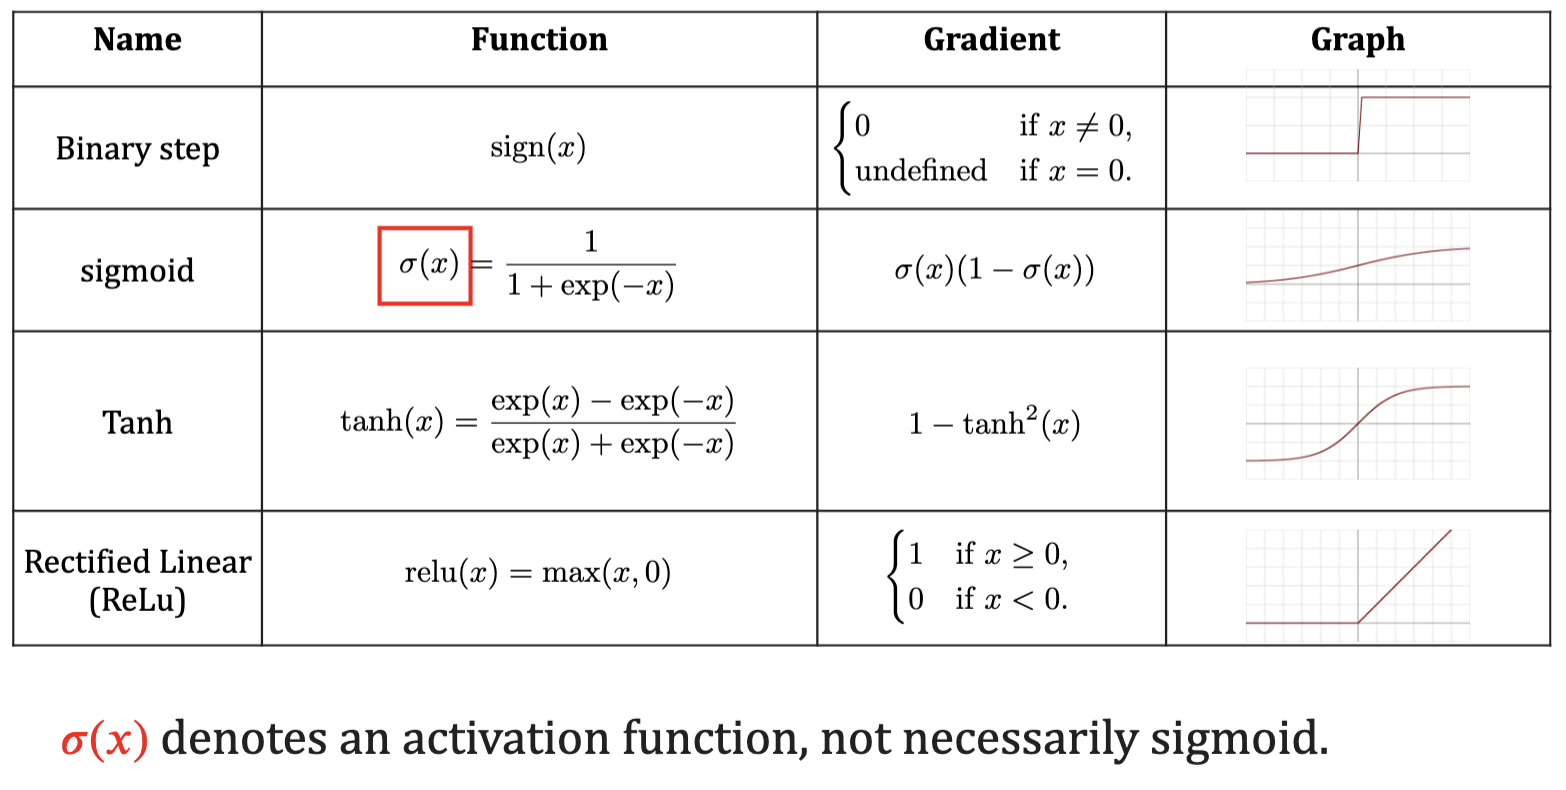
\includegraphics[width=0.6\textwidth]{Images/activations.png}
\end{center}

\begin{itemize}
    \item \textbf{Binary step:} Outputs 0 or 1, not differentiable at $x=0$.
    \item \textbf{Sigmoid:} Smooth, outputs between 0 and 1, can cause vanishing gradients.
    \item \textbf{Tanh:} Outputs between -1 and 1, zero-centered.
    \item \textbf{ReLU:} Simple, efficient, helps with vanishing gradient, but can "die" for negative inputs.
\end{itemize}

Deeper neural networks can express more complex functions only if we use non-linear activation.

If all activation functions are linear, then a multi-layer neural network is equivalent to a single-layer linear model. This is because a linear function of linear functions is still linear.

\textbf{Example:} Suppose the activation in the hidden layer is linear, $\sigma_1(x) = x$, and the output activation is non-linear, e.g., $\sigma_2(x) = \mathrm{sign}(x)$. Then, the output can be written as:
\[
v_{\text{out}} = \mathrm{sign}(\bar{w}_1 v_1 + \bar{w}_2 v_2) = \mathrm{sign}\left(\bar{w}_1(\vec{x} \cdot \vec{w} + b) + \bar{w}_2(\vec{x} \cdot \vec{w}' + b')\right)
\]
\[
= \mathrm{sign}(\vec{z} \cdot \vec{x} + \beta)
\]
where $\vec{z} = \bar{w}_1 \vec{w} + \bar{w}_2 \vec{w}'$ and $\beta = \bar{w}_1 b + \bar{w}_2 b'$.



\subsection{Universal Approximators}

A fundamental result in neural networks is the \textbf{Universal Approximation Theorem}. It states that a feedforward neural network with a single hidden layer (i.e., a depth-2 network) and a sufficiently large number of neurons (width) can approximate any continuous function on $\mathbb{R}^n$ to arbitrary accuracy, given appropriate activation functions (such as sigmoid or ReLU).

\textbf{How large does the hidden layer need to be?}
\begin{itemize}
    \item For boolean functions, the required width can be as large as $\exp(n)$, where $n$ is the input dimension.
    \item If we restrict ourselves to networks of polynomial size (i.e., width and number of parameters grow polynomially with $n$), then:
    \begin{itemize}
        \item We cannot approximate all possible functions.
        \item However, this restriction helps reduce the risk of overfitting.
        \item This tradeoff is known as the \textbf{bias-variance tradeoff}: larger networks can fit more complex functions (low bias, high variance), while smaller networks may generalize better (high bias, low variance).
    \end{itemize}
    \item Instead of fully connected layers, we can use structured networks (e.g., convolutional neural networks) to reduce the number of parameters and exploit structure in the data.
\end{itemize}


\end{document}